\section{Game Design}
\label{game:design}
Games With A Purpose (\ac{gwap}) are implemented in many fields and come in various forms. With regards to their overall game design, they tend to be graphically rich, provide simple interactions and give the player an experience of progression by scoring points, leveling players up and recognizing their effort. Additionally, the design of the game should reinforce quality measures and control the behaviour of players. Encouraging players to concentrate on the task and discourage them from malicious behaviour is crucial for quality control \cite{42}. The goal of our research study was to develop a \ac{gwap} that would serve as a tool for validating the named entity disambiguation task. The validating process should be performed at the highest quality level possible and still maintain player engagement by positively affecting their intrinsic motivation: experiencing feelings of competence, autonomy and relatedness while playing. The following subsection explore the different game elements and the corresponding game design principles used in Fastype that make this game enjoyable, fun to play and motivate players to come back and play. This results in generating large-scale annotation data for our named entity disambiguation task without players noticing what the underlying purpose of the game is.

\subsection{Onboarding}
%Onboarding 
The first impression you get when meeting somebody for the first time is usually a strong indicator that determines whether you will like the company of this new person or not. Similarly, the first impression or the first minutes of interacting with a game are the most important because a player will make a decision whether he or she will continue exploring the game. According to Zichermann et al. \cite{48}, the onboarding process is critical to a successful game. A good onboarding process leaves no other options to the player but to win. It is crucial that in this stage the player will be offered with an action at which he will not be able to fail. After having completed the initial action/task, the player should be rewarded for successfully completing it. \cite{48, 43, 48}

During the implementation of Fastype, special attention was put in designing the onboarding phase as effective as possible. Fastype has been designed as a typing game where players have to type on their keyboard as fast as possible to reach high scores and improve their typing skills. Additionally, the game requires the user to focus and memorize what they type in their keyboard and also answer quiz-like questions to get additional points, reach new levels and complete various categories. All these concepts have to be carefully revealed to the player during the onboarding stage. According to Zichermann et al. \cite{48}, the onboarding process should accomplish the following things: 
\begin{itemize}
    \item Slowly reveal the complexity of the system
    \item Positively reinforce players
    \item Avoid any action that leads to failure
    \item The game should learn something about players in order to personalize the game if necessary 
    \item All the points mentioned above have to be done within the first few minutes of the player interacting with our game
\end{itemize}

Except the points listed above, we also wanted the onboarding process to be slightly intriguing and mysterious in order to tease the player's curiosity. When entering the game site, the players are presented with a screen which requires them to know a \textit{ game secret} (See Figure \ref{fig:game-startscreen}). Having a secret comination to enter the game might potentially affect feelings of relatedness as the player will experience feelings of being part of a secret game club which allows entrance only to players who are aware of the game secret. However, the game provides a way of discovering the game secret. The only way of acquiring it and being granted with access to the game is by following a trial procedure. This trial procedure represents the onboarding process for our game. 

\begin{figure}[h]
  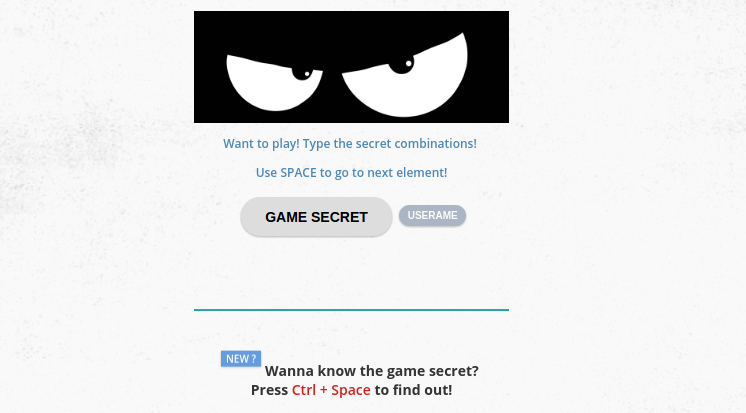
\includegraphics[width=\linewidth]{figures/experiment2/startscreen-game.png}
  \caption{The game start screen presented to player when entering the game for the first time}
  \label{fig:game-startscreen}
\end{figure}


The onboarding process starts by asking players to type the words that appear in the screen as small boxes. Points are awarded to the player regardless of their typing speed (rewarding and recognizing the players' effort). After the player is familiarized with the way the game works (typing fast while paying attention to the words that appear in the screen), the game continues by introducing a new challenge: a puzzle combined with typing skills. The puzzle consists of several hidden characters that the player has to reveal by typing the words appearing in the screen. The faster the typing the faster the revealing of characters. After the player has revealed all the characters on the puzzle, he is presented with a quiz where the \textit{question} is the revealed word (i.e. the named entity) and the options are the candidate entities extracted from \ac{kb}. Contextual clues are provided on top of the screen as sticky notes which help the player to make a correct decision. The quiz is a \textit{masked} version of the named entity disambiguation process used in the first experiment. The player proceeds by selecting a candidate option which is rewarded with 10 game points. Please note that if the player selects the wrong option, the system will not proceed until the right option is selected. As a reward for choosing the correct answer, the player finally reaches the end of the trial process where the game secret is finally revealed. Additionally, the player has to register himself with authentication credentials which together with the game secret are used as a secret combination for granting access to the game. Figures \ref{fig:onboarding}(a) to  \ref{fig:onboarding}(f) illustrate the complete onboarding process of Fastype. 

\begin{figure}[]
  \centering
  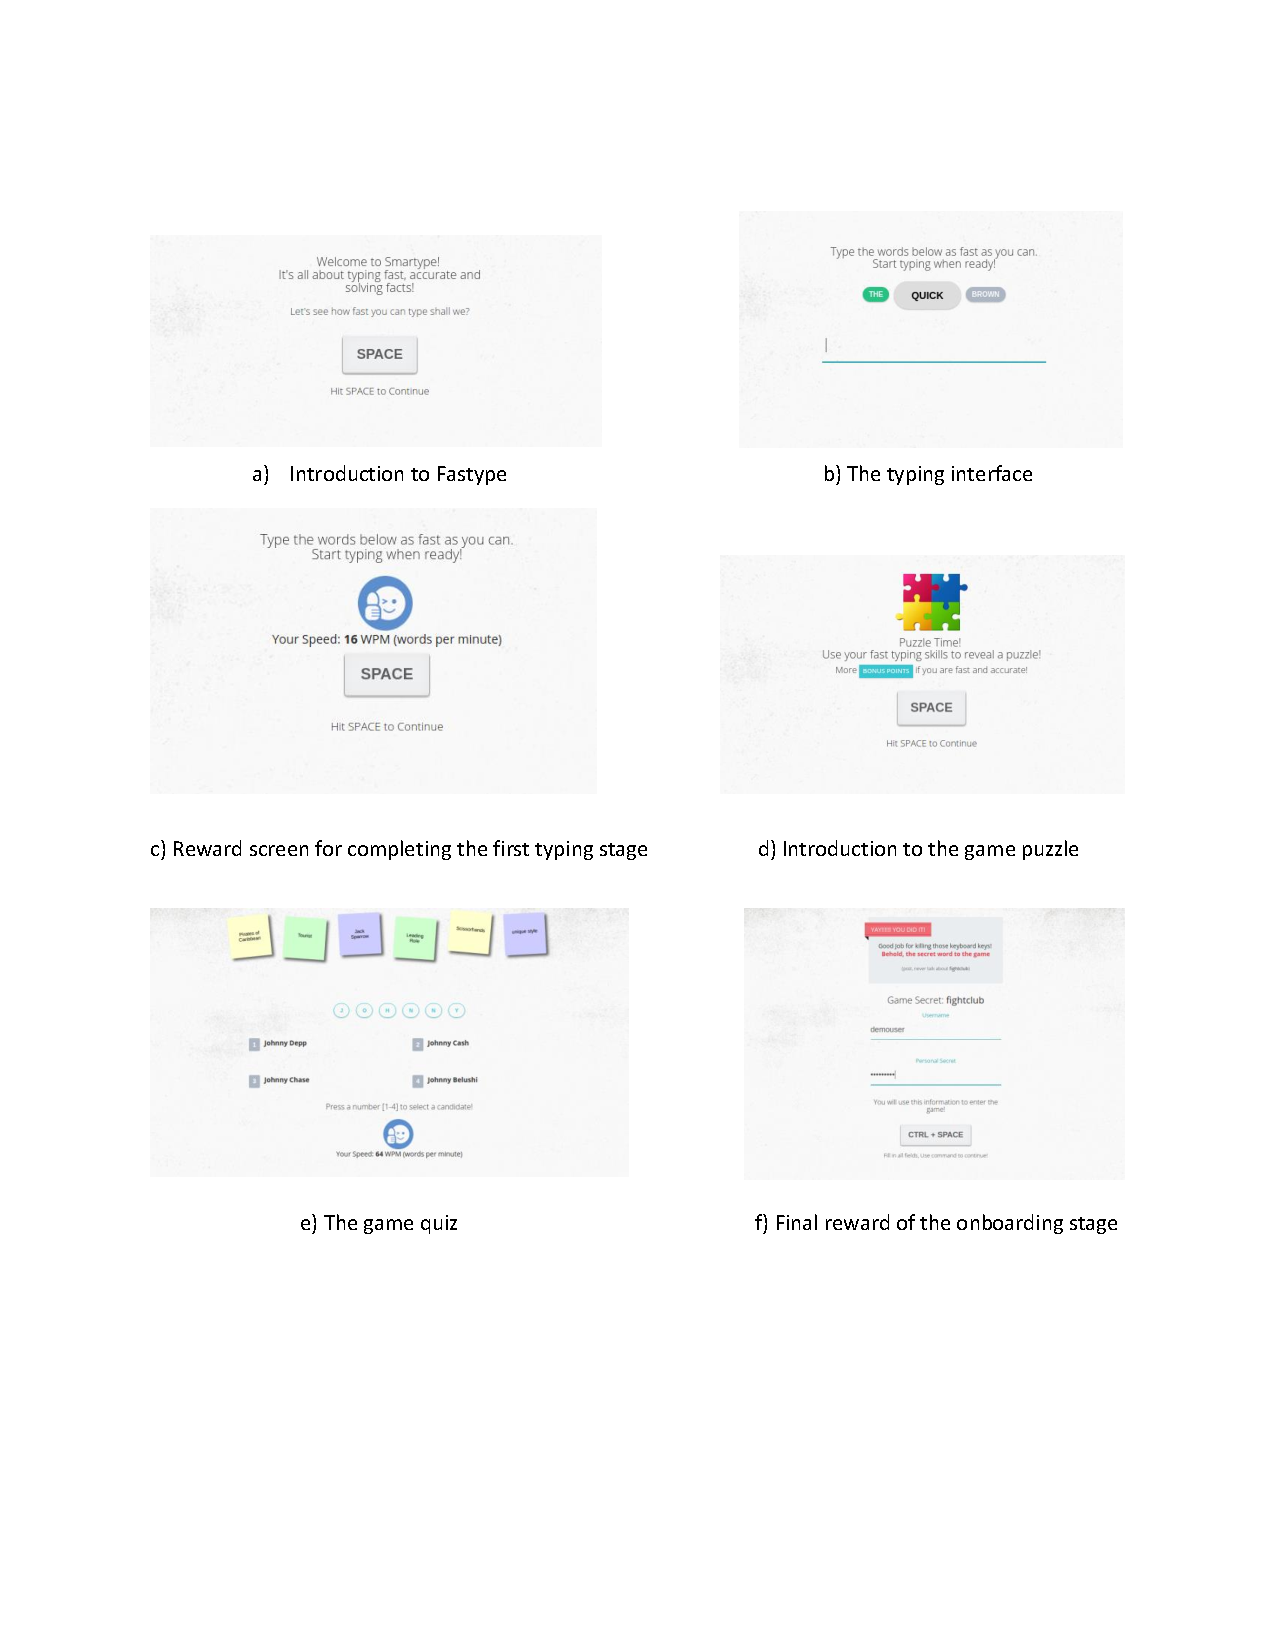
\includegraphics[page=1,width=\textwidth]{figures/experiment2/oboarding.pdf}
  \caption{The onboarding stage of Fastype}
  \label{fig:onboarding}
\end{figure}
\subsection{Task Design}
After exploring and analyzing many gamified systems and the effect of various game elements towards user engagement and motivation, Sailer et al. \cite{45} argues that gamification is not effective per se, but specific game design elements have specific psychological effects. Thus, it is important that gamification is not done just by incorporating a scoring system with some levels to advance and a leaderboard to see your progress. It takes more than that to design a game that attracts and retains a player base. 

Chamberlain et al. \cite{43} emphasizes that it is the design of the individual tasks in a gameplay that determine how successful the player can contribute data whilst playing. Furthermore, Sailer et al. \cite{45} communicates the importance of game elements being recognized by the player in the gamified environment. Delivering the treatment to the player or to a participant in the game is not enough unless the designer of the game makes sure that the treatment is also received by them. Failing to design treatments or game elements that are genuinely recognized by the players, results in loss of statistical power and risk to underestimate their effectiveness \cite{45}. In order to adhere to the aforementioned design constraints, significant work effort was placed in designing a task that contributes to generating annotation data of good quality. 


A game-round starts by the player selecting a specific category to play or letting the game choose a category in a random fashion for the player. Everything in the game is designed in a way that the player only has to use the keyboard for completing almost every action. The player is then presented with the typing screen where a combination of hidden characters have to be revealed by typing as fast as possible. Figure \ref{fig:game-typingscreen} illustrates the typing screen. A speed radar is placed right underneath the typing text box which displays the current speed of typing measured as the amount of words typed per minute while the player is revealing the hidden characters. This element can be considered a strong motivator to keep the player focused on typing fast. After having revealed the word, the upcoming challenges/questions all revolve around the text that has been typed during the typing phase. The players are already familiar with this concept since a similar task was already performed during the onboarding phase. Bonus questions are immediately presented to the user after completing the revealing stage (we talk more about the importance of bonus questions towards the overall design in a later subsection). The content of the bonus questions is created by using the text that was typed in the previous stage. Similarly, the most important part of the game that contributes to the original task of disambiguating entities is the quiz stage of the game. The quiz interface provides contextual clues extracted from our original framework and lists all the potentially candidates (quiz options) from which the player has to choose. 

\begin{figure}[]
  \centering
  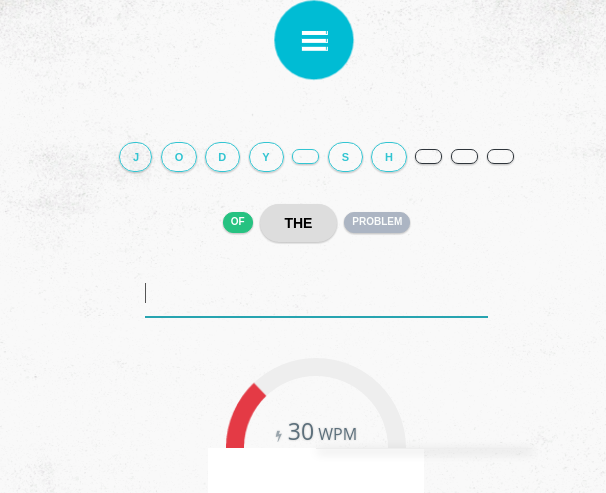
\includegraphics[width=.6\linewidth]{figures/experiment2/gameplay1.png}
  \caption{The typing screen and the speedometer calculating the typing speed of the player}
  \label{fig:game-typingscreen}
\end{figure}

We strongly emphasize the fact that all the game elements presented so far are focused and contribute to the ultimate goal, which is annotating the entity with the right candidate. The text which the player types during the typing stage, the content of the bonus questions and the contextual clues all represent carefully carved information that contribute in helping the player choose the right candidate. We make sure that the typing text\footnote{During the fast-typing stage, players are presented with different words that appear on the screen one after another. These words are part of a complete paragraph that is taken from the document where the target entity is part of.} as a game element is recognized and takes the attention of the player because if players are able to remember the text they typed, they can get points from correctly answering the bonus questions and also be confident on the candidate option they select. An example of a bonus question is presented in Figure \ref{fig:game-bonusqeustion} while the quiz interface of the game is illustrated in Figure \ref{fig:game-quiz}. 

\begin{figure}[]
    \centering
    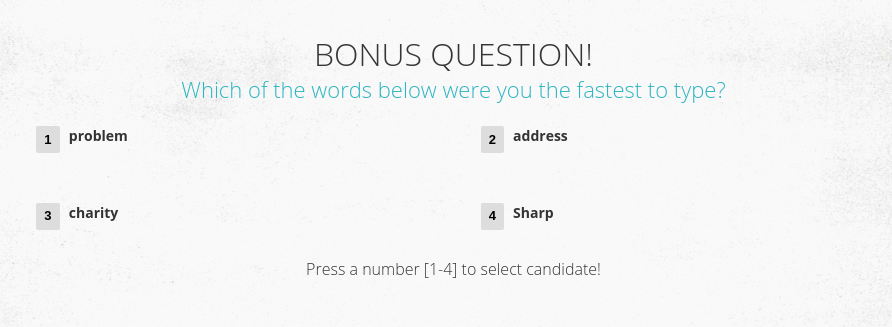
\includegraphics[width=.8\linewidth]{figures/experiment2/bonusquestion.png}
    \caption{An example of a bonus question}
    \label{fig:game-bonusqeustion}
\end{figure}

\begin{figure}[]
    \centering
    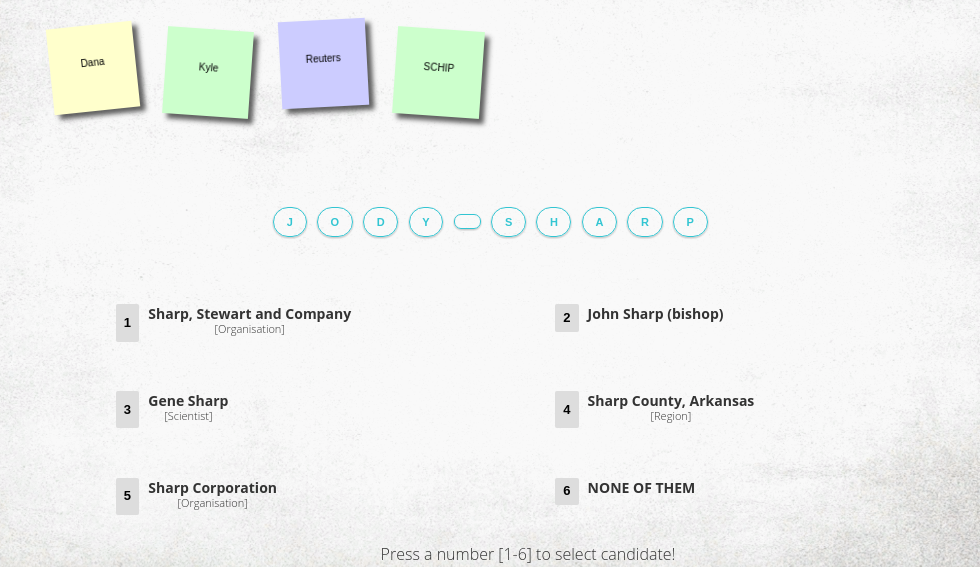
\includegraphics[width=.6\linewidth]{figures/experiment2/game-quiz.png}
    \caption{Interface of the game quiz - a gamified version for the named entity disambiguation task}
    \label{fig:game-quiz}
\end{figure}

%Skillset required/improved in the game
Schell \cite{51} (page 214) emphasizes the importance of the skill and chance mechanisms in games. A good game should balance between skill and chance during the gameplay. We believe that we have reached a satisfactory balance between these two factors by equalizing the factor of chance and skill required. The factor of luck is represented by bonus questions which are extracted from the typing text and are genuinely hard to answer since a memorization of everything typed is required. On the other hand, the factor of skills is represented by the quiz element of the gameplay. Correctly answering the quiz requires certain skill-sets from the player in order to maximize their profit point-wise. Except requiring skills from the players, the game should also contribute in allowing the players to master and perfection these skills. In general, by playing Fastype, a player will improve the following skills:

\begin{itemize}
    \item Typing skills
    \item Concentration in time pressure 
    \item Memory training and pattern recognition
    \item Knowledge in different categories (politics, music, entertainment, health etc)
\end{itemize}

Improving these skills is one of the goals that players will attempt to achieve. After having observed the players during their gamplay when conducting the second experiment we are aware that the goals of the game are concrete, achievable and rewarding at the same time. Having all these three elements characterizing the goals of the game is crucial to keeping players engaged and motivated \cite{51}. 

Reviewed literature suggests a number of criteria for evaluating enjoyment during gameplay. Some of the criteria which apply to task design and which also relate with SDT in terms of their importance towards increasing intrinsic motivation include: Feedback and Immersion \cite{41}. Constant feedback is given to the player for every performed action when interacting with Fastype. Immersion in our case refers to a short and arcade style of the gameplay which make the player experience a deep and yet effortless involvement in the game \cite{41}. A game round in Fastype lasts 4-5 minutes on average with the player being exposed to different challenging tasks. This results in an effortless and deep involvement in the game for a short period of time. Additionally, the game elements and the feedback provided during the gameplay have been enriched with sounds, visuals and animations which according to Mekler et al. \cite{46} can positively affect competence, needs satisfaction and subsequently increase intrinsic motivation.

%performance graphs, levels, leaderboards, points 
Game elements such as performance graphs, levels, points and leaderboards are provided in the game in order to give the players the feeling of progression and advancement. With these game elements we also reinforce the competitive nature of players to compete with others but also work hard on breaking their personal best scores. This results in encouraging players to get better each time they enter the game (mastery of skills). Figure \ref{fig:game-profile} illustrates the profile of the player where a performance history of the typing speed is provided in addition to level information, challenge status and betting ratio (a balance between the bets lost and won).

\begin{figure}[]
    \centering
    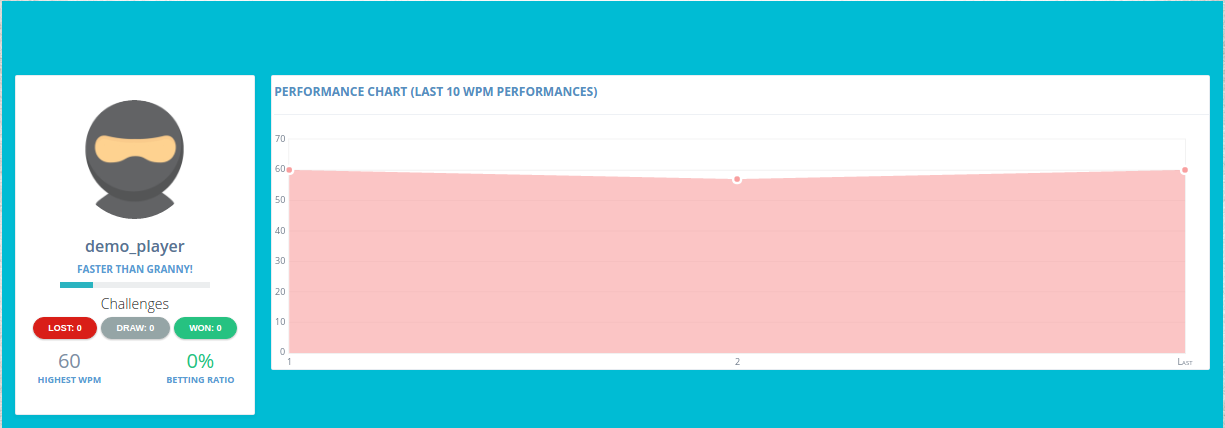
\includegraphics[width=\linewidth]{figures/experiment2/profile.png}
    \caption{Player profile screen}
    \label{fig:game-profile}
\end{figure}

The final element that requires our attention is the concept of game-flow. It was explained in the background section of this chapter that game-flow is the concept of keeping the player constantly engaged while not overwhelming him with problems that are too complex to overcome or too easy that the player gets bored quickly. Our idea of keeping the complexity of the game in the same level as the player's progression and skill improvement in the game is by increasing the total number of words that players have to type within a game-round. The complexity is controlled by the level mechanism of the game. When players progress and reach new levels, they are faced with longer and more complex paragraphs to type. However, one can argue that this is not the best and most optimal way of maintaining game complexity and player's flow zone. Being limited in the amount of resources available to be spent in designing and implementing all the game elements, the proposed idea of defining and maintaining game complexity was the only achievable concept within these constraints. However, ideas to improve the existing design of game complexity will be addressed in the discussion section and as such will be accounted for future work. 

\subsection{Freedom of choice}
%Autonomy - Freedom of choice - categories 
%training phase
During the first experiment where the non-gamified interface was used to perform annotations, many participants addressed the fact of not having control over the genre of the entities presented to them. Since the selection of the entities to be resolved was done in a random fashion, one of the participants was constantly getting entities that fell into the Arts category. As a consequence, the participant was feeling very insecure during the task because of being unfamiliar with most of the concepts being presented to him. We would like to stress out the importance of freedom of choice in this aspect. Being able to freely decide what category to play in, is an important factor for reinforcing autonomy and competence. As a result, the game gives the player the freedom of choice by providing several game categories to choose from. For players who like the aspect of surprise and chance, the game can make a random choice for the player if instructed to do so. 

Furthermore, the game provides a training phase for players who feel unprepared to take the actual task where the performance is recorded. According to Chamberlain et al. \cite{43} GWAP usually begin with a training phase so that players are able to practice their skills and also show that they have understood the instructions before they do the real task. However, in our case the onboarding stage takes care of explaining the complexity and instructions for performing actions in the game while the training phase allows the user to practice their typing skills. The training phase was also designed for the purpose of getting familiar with a new keyboard since the participants played the game from the experimenters laptop and therefore it was necessary to have a training phase. The game acknowledges the player for the existence of a training possibility in the game by pushing notification on the screen.
\subsection{Game challenges}
%Challenges 
%Punishmet
Von Ahn in his pioneering work \cite{vonahn} focuses on one type of incentive to motivate players: enjoyment. He emphasized that the main mechanism to make players enjoy a GWAP is by providing them with a challenge. Usually in many gamified systems, challenges are achieved through mechanisms such as requiring a timed response, keeping scores which ensure competition among players, having players with similar level of skill compete against each other and so on. \cite{44} 

The design of Fastype strongly reinforces the competitive nature of players by providing challenges which allow players to compete with each other. During each game round, the system keeps track of the player's typing speed, and shows potential challenges based on their WPM (Words Per Minute) accordingly. To assure fair play, the system makes sure that the player is presented with challengers that have roughly the same level of skill. The challenge screen is presented to the player after she has completed the quiz. Figure \ref{fig:game-challenge-screen} shows the exact challenge screen which is used by players to send challenge requests to other players in the game. As seen in the figure, players can choose a number of points between 1 and 10 to challenge the other players. These points represent the reward or punishment mechanism of the challenge. To assure fair play of the game, players who are challenged will type the exact same words as the challengee, therefore an accurate measure of their skill is guaranteed. Finally, having a challenging game where each challenge matches the players skill level contributes to the feeling of enjoyment during gameplay \cite{43}.

\begin{figure}[]
    \centering
    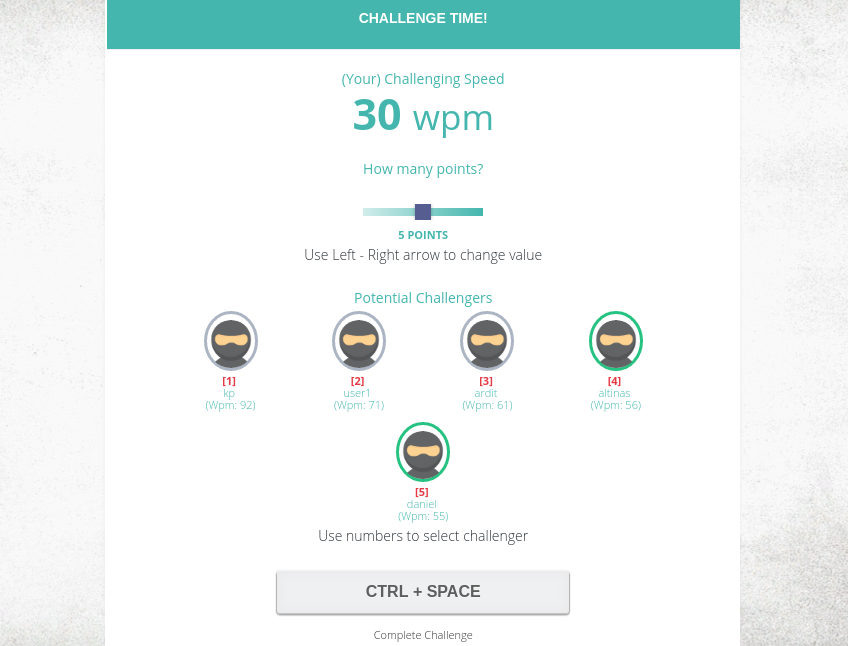
\includegraphics[width=.8\linewidth]{figures/experiment2/challenge-time.png}
    \caption{Fastype Challenge Screen}
    \label{fig:game-challenge-screen}
\end{figure}

An additional note that requires attention is the mechanism of punishment in a game. Schell \cite{51} (page 225) addresses the importance of punishment mechanisms in games and if balanced appropriately, they will give more meaning to everything in the game. Punishment mechanisms increase the value of certain game elements such as points. In Fastype, challenges and the betting mechanisms provide a way of punishment for players. In case of failure, their accumulated game points will be taken away, subsequently dragging the player down in lower levels in addition to increasing the failure percentage in their profile. Please note that the players have always the option of skipping challenges or bets on their answers. As a consequence of avoiding challenges and bets in the gameplay, the player will experience a slow progression and less dramatic gameplay as compared to other players who take risks by betting and challenging other players.
\subsection{Bonus Questions} 
%lens of chance
%the element of surprise, random nature (never know what to expect), have to rembmer all what was written and how it was written, a skill which is hard to master but interesting and misterious and with the help of chance it is sometimes easy achieved
The bonus questions represent the element of chance and surprise in our gameplay. The random nature of the bonus questions give the game a unique flavor of mystery and surprise since the player never knows what to expect from the bonus questions and therefore it encourages players to work on remembering what and how she was typing. Some bonus questions ask about the total number of words typed, the fastest word typed, the number of times a player failed to type a word correctly, the number of times a specific word occurred etc. The bonus question play an important role in the overall playfulness and feelings of enjoyment during gameplay. 
\subsection{Betting System - a measure for quality control}
Many of the existing gamified systems point out the importance of quality control in \ac{gwap}. Von Ahn et al. \cite{44} suggests two mechanisms for ensuring correctness of data: player testing \footnote{Player testing is evaluating the players output by occasionally matching it against gold standards or already annotated data} and repetition or redundancy of data. In our game design we have employed two mechanisms for ensuring that the quality of annotations performed through the game is maintained. 
The first assessment methodology is accumulating multiple individual answers for a specific entity before deciding whether that answer is correct or not. This corresponds to the redundancy of data for quality control suggested by \cite{44}. The second assessment methodology is using the betting system incorporated into the game. If we look at the betting element in the game from the eyes of a game designer, this element represents the lens of triangularity proposed by Schell \cite{51} (page 212). The lens of triangularity gives a player the choice to play safe for small rewards or take a risk and win big rewards. Triangularity gives an interesting and exciting flavour to our game. On the other hand, if we look at this game element from the eyes of a linguistic expert who demands from the game the generation of trustful and qualitative annotations, than this element represents a measure for assessing the confidence of a player towards the his choice of candidate. Figure \ref{fig:game-bet} illustrates the betting screen shown to the player immediately after having completed the quiz.

\begin{figure}[]
    \centering
    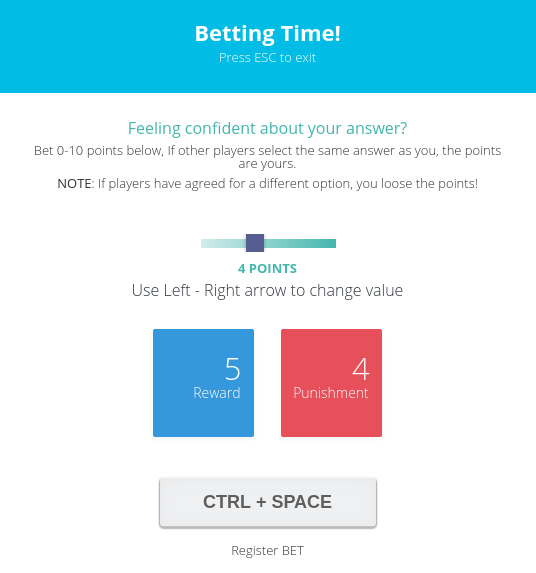
\includegraphics[width=.8\linewidth]{figures/experiment2/game-bet2.png}
    \caption{Betting Mechanism as a quality control and representative of triangularity for Fastype}
    \label{fig:game-bet}
\end{figure}

As we can see from Figure \ref{fig:game-bet}, the player has the choice of deciding the amount of points he wants to bet on the selected answer. The bigger the number of points used in the bet the higher the risk of loosing or wining them. Players are instructed to think if other players who might potentially encounter the same quiz will also choose the exact same answer as they did. In that case, if they are confident about the given answer, then the players are encouraged to place high bets rather than playing it safe. However, the choice remains completely in the hands of the player. Our betting mechanism works in the way that for one individual entity, when more than 4 unique judgments agree on the same candidate, than this entity is considered to be resolved. All the players whos' selected candidate is the same as the correct candidate (meaning their answer falls within the absolute majority) will be rewarded with the amount of points they bet for the particular entity. Similarly, all the players whos' answer was not the one selected by the majority are punished by subtracting the amount of points they bet from their overall accumulated points in the game. In terms of annotation quality, candidates with higher betting scores represent higher levels of confidence which means we can be sure that the selected candidate is undoubtedly the correct representative for the target entity.
\subsection{Social Interaction \& Engagement Loop}
%SHoutouts, challanging, desire to compete (being the first in the board) each other as relatedness factors - increasing social interaction - Relatedness is a factor that positively affects intrinsic motivation
Significant design and implementation effort was put in making the game as much socially interactive as possible. Among the three SDT elements which have direct impact in intrinsic motivation and needs satisfaction, social interaction contributes to the feeling of relatedness with others. The main social interaction mechanism implemented in the current version of the game are challenges. The desire to compete and overcome players in the leaderboard can be seen as an element that entails social interaction within the game. 

%engagement loop
The concept of engagement loop on the other hand is a fundamental aspect that needs to be clearly defined in order to maintain player motivation. A successful designed engagement loop always leaves something incomplete or pending in the game for players to come back and play. Game designer David Perry suggests that the key to addictive game design is by creating a game that keeps the player engaged by doing three things all at the time: exercising a skill, taking risks and working out a strategy \cite{15}. Zicherman et al. \cite{48} gives substantial importance to the social engagement loop and defines the following four key aspects to be considered by game designers when thinking about engagement loops: motivating emotion, player re-engagement, social call to action and visible progress/rewards. Table \ref{tab:engagement-loop} lists the game elements of Fastype that contribute to the different aspects of social engagement loop.

% Table generated by Excel2LaTeX from sheet 'Sheet1'
\begin{table}[htbp]
  \centering
  \caption{Game elements of Fastype that contribute to the social engagement loop}
    \begin{tabular}{|c|l|}
    \toprule
    \multicolumn{2}{|c|}{Social Engagement Loop} \\
    \midrule
    \multirow{Motivating Emotion} & Excercising fast typing \\
          & Competing with others \\
          & Learning new facts  \\
          & Improving Memory skills \\
    \midrule
    \multirow{Player Renegagement} & Levels \\
          & Challenges  \\
          & Increasing WPM  \\
          & Completing Categories \\
    \midrule
    \multirow{Social call to action} & \multirow{Challenges } \\
          &  \\
    \midrule
    \multirow{Visible progress} & Leaderboard \\
          & Points  \\
          & Levels  \\
          & Challenge Win/Lose Ratio \\
    \bottomrule
    \end{tabular}%
  \label{tab:engagement-loop}%
\end{table}%